\documentclass{article}
\usepackage[utf8]{inputenc}
\usepackage{xcolor,listings}
\usepackage{textcomp}
\usepackage{subfig}

\lstset{upquote=true}

\title{LINGI2132 : IoT network using Rime}
\author{Roussieau Julian - Desausoi Laurent - Minet Jeremy}
\date{\today}

\usepackage{natbib}
\usepackage{graphicx}
\usepackage{paralist}
\usepackage{varwidth}

\begin{document}

\maketitle

\section{General structure}

Our IoT network is divided in two main parts. As shown on figure \ref{network}, the right-hand side corresponds to the sensor network composed of multiple embedded systems (Z1, Re-Mote or Firefly) communicating together via \textit{IEEE 802.15.4}. In this network, one node has been elected with the \textbf{root} status and is responsible for gathering and forwarding the data to the MQTT-Rime gateway. The binding between this node and the gateway is made via serial port. In the real life, this would simply by a physical cable but since we are working in a virtualized environment, we have emulated this link by installing the \textit{serial2pty} plugin in order to enable the bridge. The gateway can be seen as a normal computer being part of the MQTT network. All these components communicate together like a normal IP network using the MQTT protocol. 

\begin{figure}[!h]
   \includegraphics[scale=0.5]{iot_network.png}
   \caption{\label{network} IoT network}
\end{figure}

\section{Network organization and routing in the sensor network}

Our sensor network is, as requested, tree-shaped. It means that on top of the structure, we find a root node that as been manually set up to be connected to the outside world, here with the gateway. All the other sensors in the network are normal nodes. Here below we explain how we construct the tree.

\subsection{Routing}

Something that one should know is that all nodes in the network are always listening to new messages, but no always sending. Indeed, a node never transmits data if it is not connected to the root. By "connected to the root" we don't mean \textit{directly} connected to the root, but rather has a path leading to the root node. So the routing begins at the root level. It first broadcasts a \textit{DISCOVER} message with its distance to root (here thus set to 0 since it is itself). Every node being listening, the ones that are in the root scope get the message and compare the distance received (computed in number of hops) in the message with their own, initially set to -1. If the path length is better, they update their inner value, retain their parent from which they received the information and retransmit the broadcasted message with the hop-value incremented by one. The process is repeated until every node in the network find a path to the root. Of course, the nodes that cannot by reach by any other nodes in the network are left apart if not moved later, in that case they will receive a \textit{DISCOVER} message after some time since the nodes are permanently sending discovering messages. Sending those messages at regular intervals allows to update the tree if better paths can be found in case of, for example, some nodes are moving and shutting down. It also acts like \textit{Keep-Alive} message for stationary nodes since each of them maintain a timer that expires if no message are received after a certain amount of time from their parent (representing the connection to the root). This could appear if a parent node becomes unavailable, requiring to find a new parent node. The other utility of the new discoveries is to allow new nodes to join the network without having to recompute the whole, they simply join the best auxiliary to the root node.

\subsection{Data transmission}

Once the whole tree has been constructed, the connection is set on both direction. In addition to the regular \textit{DISCOVERY} messages preserving the routing, data messages are also send. Upward, the sensor nodes send their measurements to the root. Downward, the root propagates the instructions received by the MQTT-Rime gateway.\\
The sensor nodes send their data to their own parent via unicast. Each parent relays the information according to the same protocol towards the root. Unicast messages are used since they are less consuming, more reliable and of course because they only target the parent node, not the entire network. 
\\
On the other side, the gateway can send configuration messages to the root node that has to forward them down the tree. We had to make a choice between unicast and broadcast for this downward transmission, and we eventually opted for the broadcast alternative. We know that doing this, we loose the reliable advantage of unicast but our decision was motivated by the following scenario : imagine a large number of sensor nodes at the first level of the tree. Sending a unicast message to every child of the root would be very consuming, while a broadcast would only need to be sent once in order to be received by all nodes. Since the embedded systems used in this IoT network have restricted resources, the broadcast solution appears more appropriate for us.


\section{Message format in the sensor network}

In the sensor network, messages are exchanged in two directions : from the sensors to the root (upward) and from the root to all sensor nodes (downward).
\subsection{Downward communication}
Concerning the latter communication, the messages broadcasted downward the tree have a structure containing two fields, a type and a data (depending on the type), both being integers in order to decrease as much as possible the size of the transmitted information. We distinguish three types of messages and their corresponding integer value: \\
\underline{\textbf{DISCOVER - int 0}} : used during the routing for the tree-shaped construction of the sensor network. The data embedded is the number of hops towards the root. \\
\underline{\textbf{CONFIG - int 1}} : used to specify new configuration options that the network should apply. The data carried out represents the mode of transmission that the core nodes should respect : 0 for periodic sendings and 1 for on-change signaling.  + POWER OF considérer aussi comme message de config ??????\\
\underline{\textbf{SIGNALLOST - int 2}} : used when a node lost its connection to the root. By sending this broadcast message, it warns all its children that they cannot reach root anymore by sending through him. There is no data for this kind of messages.

\subsection{Upward communication}

For the unicast communication going from the core nodes to the root, the message is a string of the following format : \\
\begin{center}
\centerline{\textit{node\_id/topic:value}}
\end{center}
A possible example looks like this : \\
\begin{center}
\centerline{\textit{4/0:-17}}
\end{center}
This message has been sent by a sensor identified by the id 4 concerning the temperature with a value of -17 degree Celsius. We decided to make a matching between the real name of the topic and an integer in order to minimize the amount of data sent in the sensor network. The gateway is responsible for making the translation between this notation and the explicit topic name on which the MQTT clients have subscribed. \\
We have two different types of send. They are both dependent on the same timer, when this one expires the data is sent if the mote is in periodic mode. On the other hand if the mote is in mode onChange, the data will be sent only if they have changed since the last sending.
\\
\textit{N.B.: For experimentation, we have created only two different topics (temperature and humidity). Each node can send both with a randomly generated value in the interval \textbf{[-10;39[} for temperature and \textbf{[0;100[} for humidity.}

\section{Optimizations}

\subsection{Stop sending if there is no subscriber}

In order to save energy and network bandwidth, we decided to stop sending data to the MQTT broker when no subscription are active anymore. Doing this requires that the MQTT-gateway becomes not only a publisher but also a subscriber. Indeed, making him listen to the status log topic about the number of active subscriptions allows us to directly send a warning message to the root node when the counter drops to 0 (in fact it is 1 since the gateway himself is an active subscriber). The root then broadcasts the configuration message telling all the nodes to stop sending data.

\subsection{Aggregate messages}

In our IoT network, we have implemented two different kind of forwarding methods : it can either be one-by-one, meaning that each node will transmit the received data one after another, or either by aggregation, storing intermediate results and sending them together afterwards.\\
If the aggregation option is activated, each time a node receive something from one of its children, it will check the two following conditions :
\begin{itemize}
    \item if the size of the buffer + the size of the received data exceeds 100 bytes, then we forward the current content of the buffer, flush it and append the new data (the maximum buffer size is constraint by the maximum packet size in Rime).
    \item if the aggregation timer has expired, we also send and flush the content of the buffer before adding the new data. The timer has been set to two minutes in order not to be to frequent and largely exceed the normal transmission timing of 16 to 32 seconds. We also add between 0 and 20 seconds to this two minutes to make sure that all aggregates are not sent together and to enable the possibility for some aggregates to be received and appended to another message before it is sent. Doing this allows to decrease the number of simultaneous communications.
\end{itemize}
 If both conditions are negative, we simply append the data to the current buffer and set it upon the next match over these conditions.

\section{Measurements}

In order to see the performance and stability of our implementation, we made some measurements for different network configurations using PowerTrace. For each, we measured the mean CPU utilization and power consumption in Lower Power (LPM), Transmit (TX) and Receive (RX) states of the sensor nodes. \\
As it can be seen on figure \ref{g1} in annexes, when the aggregation option is set, the number of nodes in our network doesn't have any real impact. Indeed, all the metrics stay the same. This is quite logical since the nodes are only sending the aggregates on a regular basis. Therefore, their power consumption is reduced.\\
On the other hand, when looking at figure \ref{g2} corresponding to default mode, it can clearly be seen that the average consumptions are increasing with the size of the network. This can be explained by the fact that all nodes are sending together whenever they want and don't care about synchronization.\\
Last thing to notice is that, even for a small number of nodes, the average power consumption is clearly higher in default mode, justified by the number of simultaneous communications. For a 10 nodes network, the power consumption in the first case is around 1 mW and more than the double in the second case.
\section{Annexes}

\begin{center}
\begin{figure}[!h]
   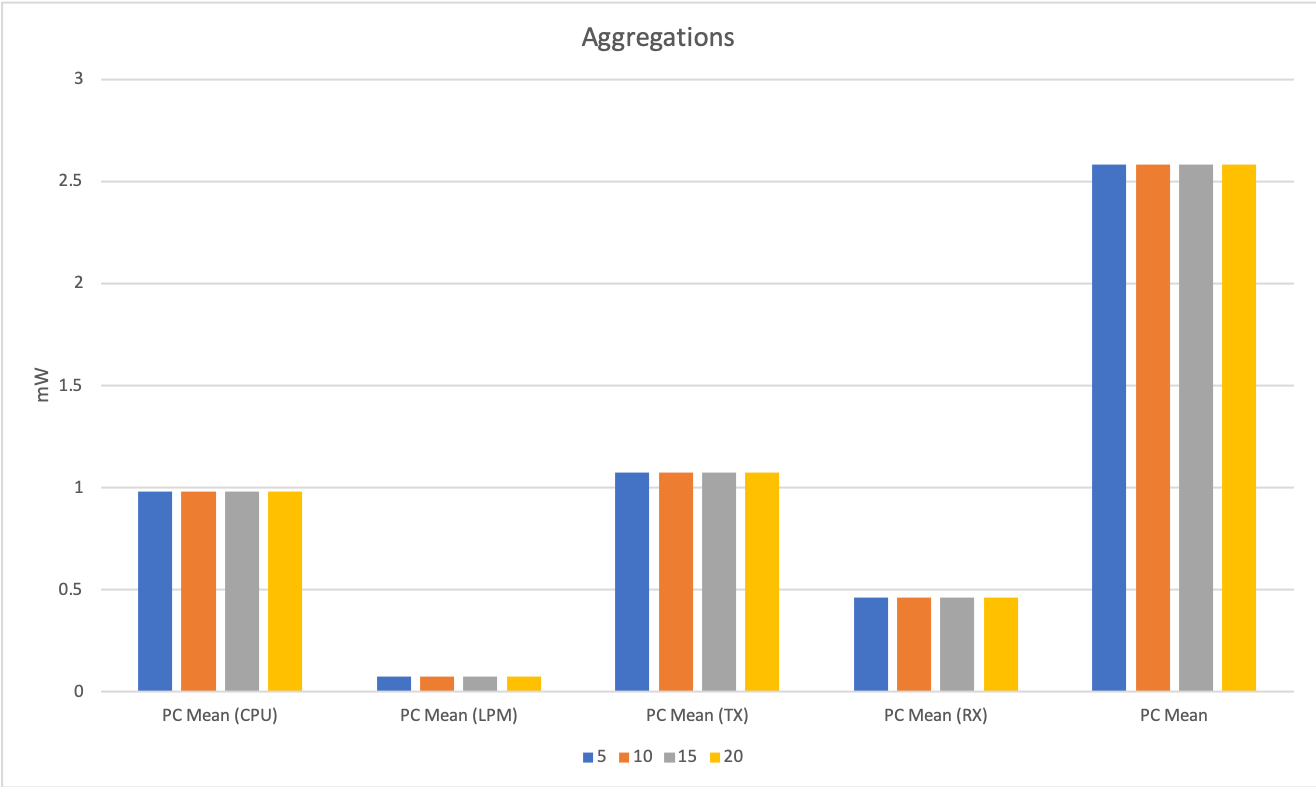
\includegraphics[scale=0.5]{aggregation_graph.png}
   \caption{\label{g1} Aggregations}
\end{figure}
\end{center}

\begin{figure}[!h]
   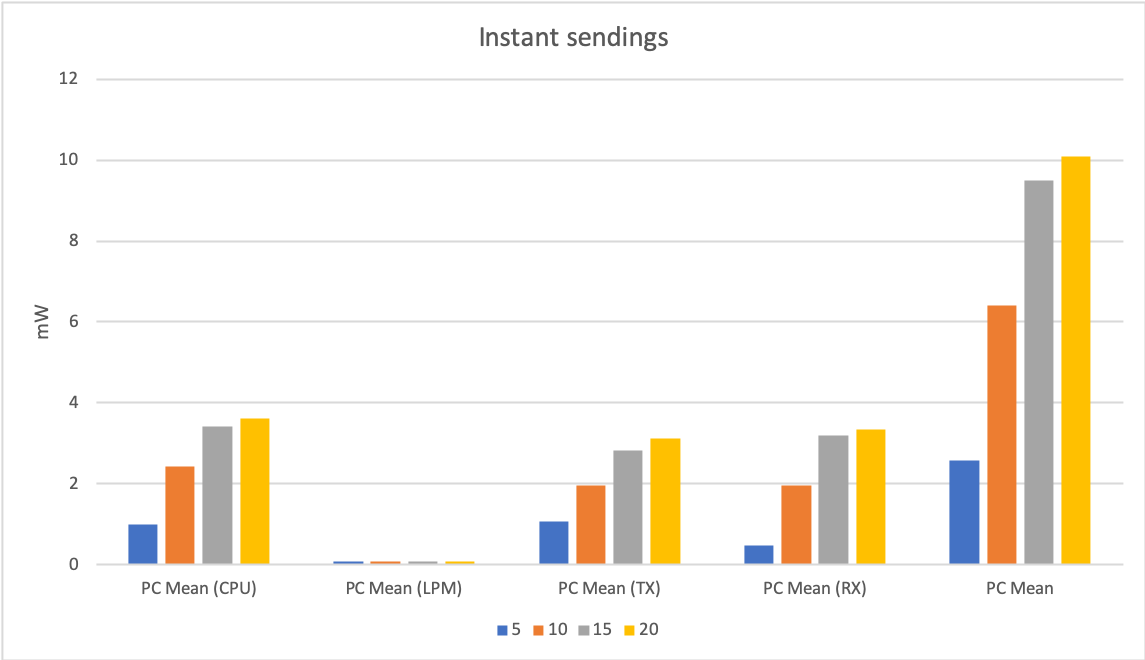
\includegraphics[scale=0.6]{instant_gaph.png}
   \caption{\label{g2} Instant sendings}
\end{figure}

\end{document}
